%
% Messageversand:
% Busimplementierung codiert Nachricht
% -- In LLZ-Protokoll als Datenversand (REQ)
% -- IN LLO-Protokoll als Datenversand (STX) mit Sequenzzaehler
% in seriellem Transferprotokoll
% Transfer ueber RS232C-Schnittstelle
% Decodierung auf ``Proxy''
% Unmittelbare Recodierung auf MCP2510 CAN-Controller und Transfer ueber ``dominante''
%%% CAN-Message
% Empfang der Botschaft auf allen horchenden Zielgeraeten bei explizitem Polling
% Decodierung gemaess LLO-Protokoll
% Acknowledge gemaess LLO-Protokoll fuer CAN-Bus schedulen
% Decodierung gemaess LLZ-Protokoll
% -> Ist Datenversand!
% 
%
%
%
% Rueckantwort: SX codiert Nachricht in LLZ (NTF) als Notifikation und in
%%% LLO (RTX) als Datenversand von der Peripherie
% SX versendet Nachricht, Proxy ACKnowledged
% Proxy codiert Botschaft (unueberprueft) in seriellem Transferprotokoll
% PDA empfaengt und dekodiert Botschaft in Message-Objekt

\overlays{1}{
  \begin{slide}{Codierung der Nachricht}
    \begin{minipage}{8cm}
      \begin{itemize}
      \item{Bus-Implementierung codiert Nachricht in drei Protokollschichten:
 	\begin{enumerate}
 	\item{{\bf LLZ} (Session) als \emph{Request}}
 	\item{{\bf LLO} (Transfer) als \emph{Transfer}}
 	\item{{\bf SLP} (Seriell) als \emph{Block}}
 	\end{enumerate}
      }
      \item{Versand \"uber serielle Schnittstelle an \emph{Proxy}}
      \end{itemize}
    \end{minipage}
    \begin{minipage}{2cm}
      \begin{center}
	\includegraphics[width=3cm]{protoblock1.eps}
      \end{center}
    \end{minipage}
  \end{slide}
}

\overlays{1}{
  \begin{slide}{Nachrichtentransfer}
    \begin{itemize}
      \item{{\bf LLZ}-Protokoll
	\begin{itemize}
	  \item{Initialisierung}
	  \item{``Synchrone'' Kommunikation}
	\end{itemize}
      }
      \item{{\bf LLO}-Protokoll
	\begin{itemize}
	  \item{Ger\"ateadressierung}
	  \item{Erkennung von Fehlern}
	\end{itemize}
      }
      \item{{\bf SLP}-Protokoll
	\begin{itemize}
	  \item{Blockaufteilung f\"ur serielle Kommunikation}
	  \item{$\leftrightarrow$ Proxy-Platine (CAN-Bus-Master)}
	\end{itemize}
      }
    \end{itemize}
  \end{slide}
}

\overlays{1}{
  \begin{slide}{Nachrichtentransfer (Schema)}
    \begin{center}
      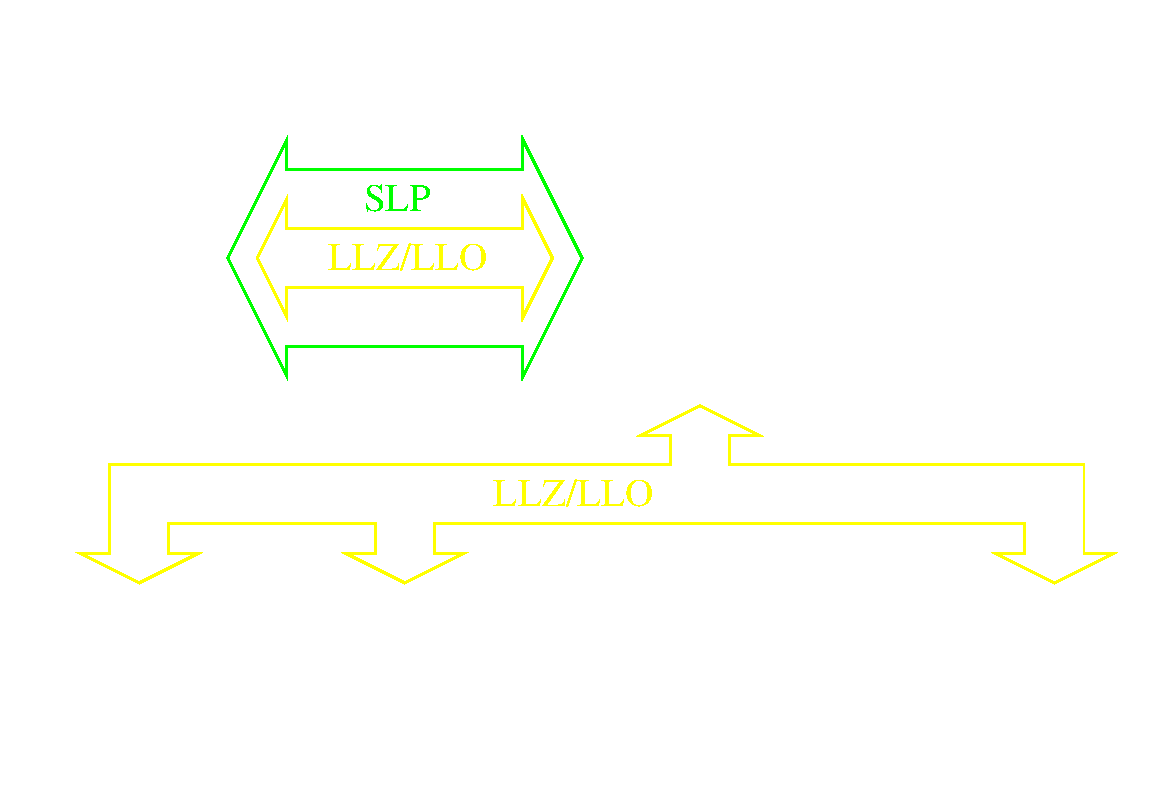
\includegraphics[width=9cm]{peripherie.eps}
    \end{center}
  \end{slide}
}

